% ================================================================
% Use the following if all authors are from the SAME institution
% ================================================================
\documentclass[accepted,single]{gipaper}

% use Times fonts
\usepackage{times}
% make sure English hyphenation rules, etc. loaded
\usepackage[english]{babel}
% permits inclusion of PNG, JPG, and PDF files under pdflatex
\usepackage{graphics}

\usepackage{epsfig}
\usepackage{newalg}

% a more flexible replacement for "verbatim" for typesetting pseudocode
\usepackage{alltt}
% gives automatic table of contents, permits setting PDF
% attributes of document.   Set page size in pdftex.cfg file;
% the "letterpaper" option to hyperref is unreliable...
\usepackage[
    pdftitle = "{Paper Format for CPSC 502/503/601}",
    pdfauthor = "{Your Name}"
]{hyperref}

\title{Paper Format for CPSC 502/503/601 \\ Instructions to Authors}

\newauthor{mm}{Your Name}{}
% Can add more authors
%\newauthor{se}{Someone Else}{}
%\newauthor{ya}{Yet Another}{}
%\newauthor{fa}{Fourth Author}{}

% Common affiliation
\affiliation{
    Department of Computer Science \\
    University of Calgary
}

% ================================================================
% Use the following if the authors are from MULTIPLE institutions
% ================================================================
%
% \documentclass[accepted,oneeach]{gipaper}
% \usepackage{graphics}
% \usepackage{hyperref}
%
% \title{Paper Format for CPSC 502/503/601 \\ Instructions to Authors}
%
% \newauthor{wd}{Author One}{Department of Computing Science\\ University of Nowhere}
% \newauthor{se}{Someone Else}{Another Department\\ A Company}
% \newauthor{ya}{Yet Another}{Yet Another Department\\ Another University}
% \newauthor{fa}{Fourth Author}{Department of Computing Science\\ University of Nowhere}
%
% ================================================================
% The rest of the document follows.
% ================================================================

\abstract{ Your text here... }

\begin{document}
\begin{keywords}
Author instructions, layout, paper formatting, electronic submissions.
\end{keywords}

%------------------------------------------------------------------
% Sections, subsections, subsubsections...
%------------------------------------------------------------------

\section{My Section}
\label{mysec}

Your text here...

\subsection{My Subsection}
\label{mysubsec}

Your text here...

\subsubsection{My Subsubsection}

Your text here...


%------------------------------------------------------------------
% Equations
%------------------------------------------------------------------

\section{Equations}
\label{equations}

Displayed equations should be numbered only if they are referenced
(in the final printing; for the review copy, number everything if
you can).   For instance, this equation is not referenced again:
\begin{eqnarray*}
    f(x) &=& \cos(x).
\end{eqnarray*}
These two, however,
\begin{eqnarray}
    g(x) &=& \sin(x),    \label{eq1}
    \\
    h(x) &=& f(x) g(x),  \label{eq2}
\end{eqnarray}
are referred to as Equation~\ref{eq1} and Equation~\ref{eq2}.

Equations should be punctuated as if they were phrases, with
commas between multiple equations. However, the only verb in a
sentence should not be the ``$=$'' sign in an equation.   Do not
begin a sentence with a numeral or a mathematical symbol.   Don't
say ``$E=mc^2$ is an interesting equation''; say instead ``The
equation $E=mc^2$ is interesting''.


%------------------------------------------------------------------
% Bibliography and Citations
%------------------------------------------------------------------

\section{Bibliography and Citations}
\label{bibcit}

Refer to citations using a square-bracketed numeral
\cite{Sousa_etal_CGF:2003}. Multiple citations should be
referenced with a comma-separated list inside brackets
\cite{Gauss:1827,Gray:1997,Shary:2002}.   Try to list such
citations in numerical order.  Citations are not nouns! They
should be treated grammatically as parenthetical statements. Say
``Consider the work of Markosian et al \cite{Markosian:1997} and
Gooch et al.~\cite{Gooch_etal_TOG:2004} '', not ``Consider the
work of \cite{Markosian:1997} and \cite{Gooch_etal_TOG:2004}''. Do
not start a sentence with a citation.

%------------------------------------------------------------------
% Algorithms
%------------------------------------------------------------------

\section{Algorithms}
\label{algorithms}

The package~\emph{newalg.sty} contains the definitions that are
needed to typeset code algorithms in a pretty way.  The Formatted
algorithms follow the style set forth in the book ``Introduction
to Algorithms'' by Corman, Leiserson and Rivest. Read the
file~\emph{newalg.pdf} for instructions and examples. Three
examples are given next.

\vspace{0.4cm}

% ~~~~~~~~~~~~~~~~~~~~~~~~~~~~~~~~~~~~~~~~~~~~~~~~~~
% Algorithm: UpdateEB
% ~~~~~~~~~~~~~~~~~~~~~~~~~~~~~~~~~~~~~~~~~~~~~~~~~~

\begin{algorithm}{UpdateEB}{i, j, facing, I_{L}}
\begin{IF}{facing = FRONT}
update~bit~fields~EB(i,j).(F, Fa) \\
\begin{IF}{I_{L} > -1.0}
EB(i,j).I_{0} \= EB(i,j).I_{0} + I_{L}
\end{IF}
\ELSE update~bit~fields~EB(i,j).(B, Ba)
\end{IF}
\end{algorithm}


\vspace{0.15cm}

% ~~~~~~~~~~~~~~~~~~~~~~~~~~~~~~~~~~~~~~~~~~~~~~~~~~
% Algorithm: LightFrontBackFacing
% ~~~~~~~~~~~~~~~~~~~~~~~~~~~~~~~~~~~~~~~~~~~~~~~~~~

\begin{algorithm}{LightSilhouettes}{mesh, origin, p_{light}, \theta}
\begin{FOR}{each~triangle~T~\in~mesh}
extract~vertex~indices~(a, b, c)~of~T \\
D \= origin - p_{light} \\
L \= v_{a} - p_{light} \\
\gamma = \cos^{-1}(D \cdot L) \\
\begin{IF}{(\gamma \leq \theta)~and~(L . N < 0.0)}
      compute~I_{L} \\
      I_{L} \= I_{L} / 2.0\\
      UpdateEB (a, b,~FRONT,~I_{L})\\
      UpdateEB (b, c,~FRONT,~I_{L})\\
      UpdateEB (a, c,~FRONT,~I_{L})
\end{IF}
\end{FOR}
\end{algorithm}

\vspace{0.15cm}

% ~~~~~~~~~~~~~~~~~~~~~~~~~~~~~~~~~~~~~~~~~~~~~~~~~~
% Algorithm: StrokeWeight
% ~~~~~~~~~~~~~~~~~~~~~~~~~~~~~~~~~~~~~~~~~~~~~~~~~~

\begin{algorithm}{StrokeWeight}{p_{1}, p_{2}, t_{1}, t_{2}, s, \alpha, \beta, N}
s \= s *(|ab|/lmax)\\
\begin{FOR}{pt \= 0~to~1,~step \= 1/res}
nib \= p_{1} + pt * (p_{2}~$-$~p_{1}) \\
t \= t_{1} + pt * (t_{2} - t_{1}) \\
r \= |PerlinNoise1D(t, \alpha, \beta, N)| \\
fill~nib~circle~at~(x,y,z)~with~radius~r
\end{FOR}
\end{algorithm}


%------------------------------------------------------------------
% Tables
%------------------------------------------------------------------

\section{Tables}
\label{tables}

Two examples of tables are given next.

% ~~~~~~~~~~~~~~~~~~~~~~~~~~~~~~~~~~~~~~~~~~~~~~~~~~
% Table 1
% ~~~~~~~~~~~~~~~~~~~~~~~~~~~~~~~~~~~~~~~~~~~~~~~~~~

\begin{table}[th]
\begin{center}
\begin{tabular}{ lrlr }
Measurement & mm & inches & pts \\
\hline
Paper width     & 215.9 & 8.5    & 612 \\
Paper height    & 279.4 & 11    & 792 \\
\hline
Left margin     & 25 & 1      & 72 \\
Right margin    & 25 & 1      & 72 \\
Top margin      & 25 & 1      & 72 \\
Bottom margin   & 30 & 1.25   & 90 \\
\hline
Column width    & 80 & 3.125  & 225 \\
Between columns &  5 & 0.25   & 18 \\
\hline
\end{tabular}
\end{center}
\caption{Paper size and margin settings.} \label{tab1}
\end{table}

% ~~~~~~~~~~~~~~~~~~~~~~~~~~~~~~~~~~~~~~~~~~~~~~~~~~
% Table 2
% ~~~~~~~~~~~~~~~~~~~~~~~~~~~~~~~~~~~~~~~~~~~~~~~~~~

\begin{table}[htpb]
\label{timings}
\begin{center}
\begin{small}
\begin{tabular}{lrlcccc}
%\hline
$\triangle$~mesh & $edges$ & {\em PP} & {\em L} & {\em W} & {\em P} & {\em W+P}\\
%$\triangle$~mesh & $edges$ & {\em PP} & {\em L} & {\em W} & {\em P} \\
\hline
Inner ear          &  16,373 & $<$ 1 & $<$ 1 &  1 &  3 & 10   \\
Pelvis/hands       &  42,231 &   1 &   1 &  7 & 14 & 27   \\
Skull              &  49,133 &   1 &   1 & 10 & 27 & 45   \\
Dental arcade      & 118,999 &   2 &   2 & 20 & 42 & 70   \\
Igea artifact      & 136,484 &   2 &   2 & 25 & 57 & 94
\end{tabular}
\end{small}
\end{center}
\caption{Average times (in seconds) for pre-processing and
rendering the models presented in this paper.}
\end{table}


%------------------------------------------------------------------
% Figures
%------------------------------------------------------------------

\section{Figures}
\label{figures}

Save your figures in PNG format. Store your result figures in the
folder at~\emph{./figs/res/} and all other figures (diagrams,
charts, etc.) in the folder at~\emph{./figs/}.

% ~~~~~~~~~~~~~~~~~~~~~~~~~~~~~~~~~~~~~~~~~~~~~~~~~~
% Figure 1
% ~~~~~~~~~~~~~~~~~~~~~~~~~~~~~~~~~~~~~~~~~~~~~~~~~~

\begin{figure}[htpb]
\centering
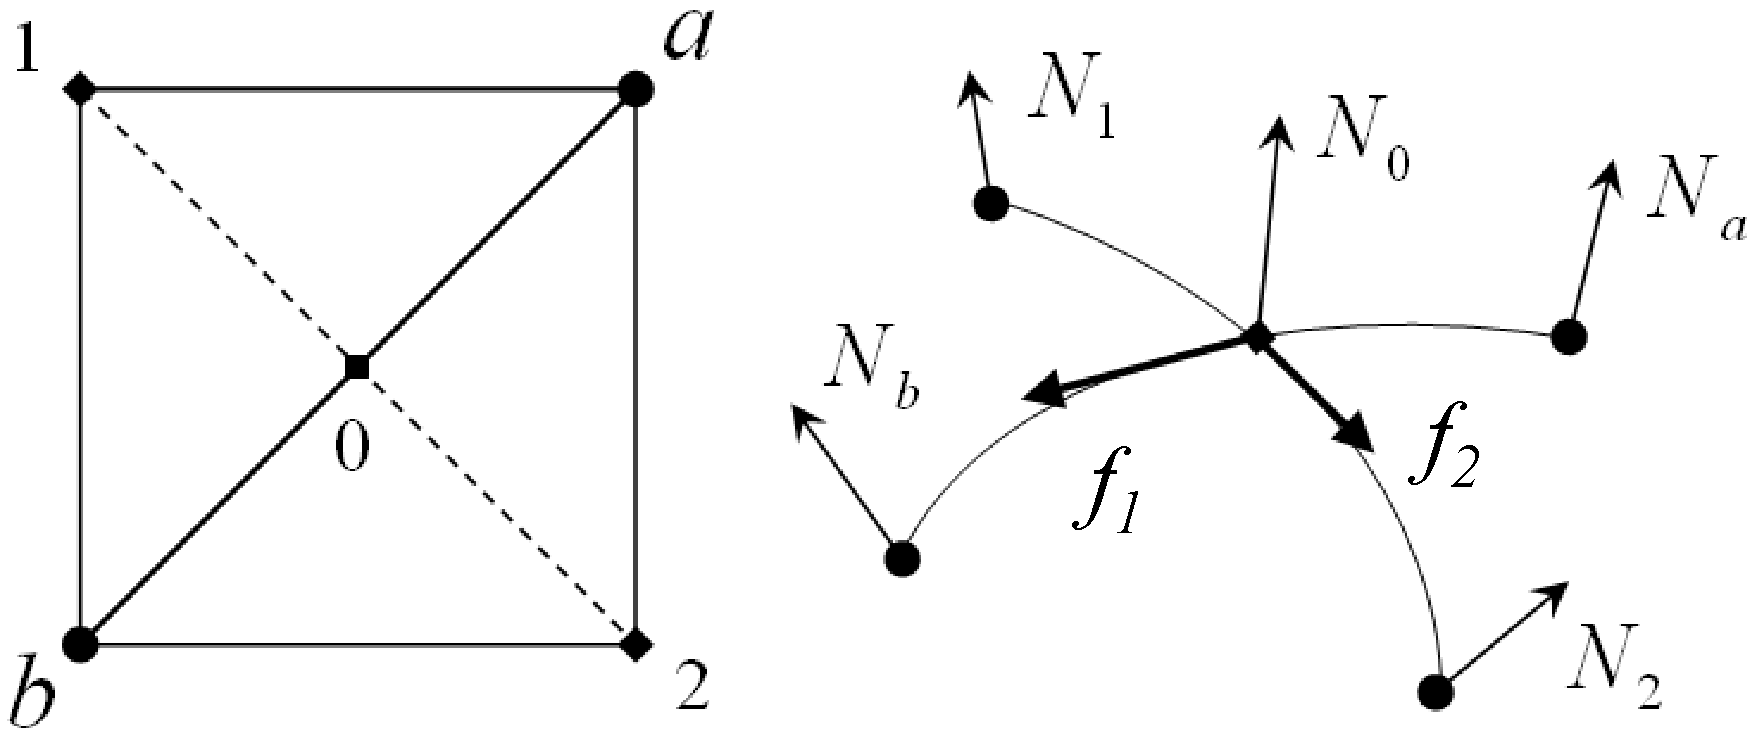
\includegraphics[width=3in]{figs/diagram.png}
\caption{
    Estimating stroke directions. } \label{fig1}
\end{figure}

A \emph{label} command appearing in ordinary text assigns to the
key the number of the current sectional unit; one appearing inside
a numbered environment assigns that number to the key. The
\emph{ref} command produces the number of the sectional unit,
equation number, ... of the corresponding \emph{label} command.
For example, anywhere in your paper, say, ...in
section~\ref{mysec}, our system computes the mean curvature
(sec.~\ref{mysubsec}), but using a different approach as presented
in section~\ref{tables} and also in section~\ref{figures}... You
can use labels for equations, figures, tables.

% ~~~~~~~~~~~~~~~~~~~~~~~~~~~~~~~~~~~~~~~~~~~~~~~~~~
% Figure 2
% ~~~~~~~~~~~~~~~~~~~~~~~~~~~~~~~~~~~~~~~~~~~~~~~~~~

\begin{figure}[htpb]
\centering
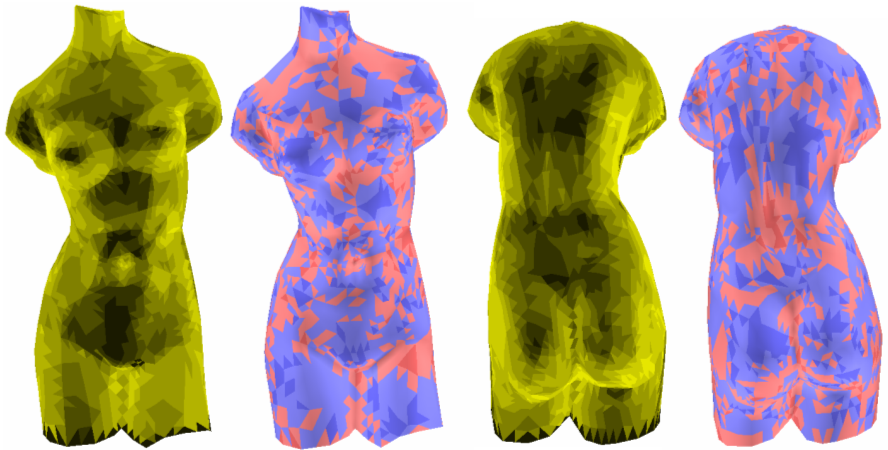
\includegraphics[width=3in]{figs/venus.png}
\caption{
    Shape measures of the Venus model~\cite{Sousa_etal_CGF:2003}.
} \label{fig1}
\end{figure}

Your text here...Your text here...Your text here...Your text
here...Your text here... Your text here... Your text here... Your
text here... Your text here... Your text here... Your text
here...Your text here...Your text here...Your text here...Your
text here... Your text here... Your text here... Your text here...
Your text here... Your text here...Your text here...Your text
here... Your text here... Your text here...Your text here... Your
text here... Your text here... Your text here...Your text here...

Your text here...Your text here...Your text here...Your text
here...Your text here... Your text here... Your text here... Your
text here... Your text here... Your text here... Your text
here...Your text here...Your text here...Your text here...Your
text here... Your text here... Your text here... Your text here...
Your text here... Your text here...Your text here...Your text
here... Your text here... Your text here...Your text here... Your
text here... Your text here... Your text here...Your text here...

% ~~~~~~~~~~~~~~~~~~~~~~~~~~~~~~~~~~~~~~~~~~~~~~~~~~
% Figure 3
% ~~~~~~~~~~~~~~~~~~~~~~~~~~~~~~~~~~~~~~~~~~~~~~~~~~

\begin{figure}[htpb]
\centering
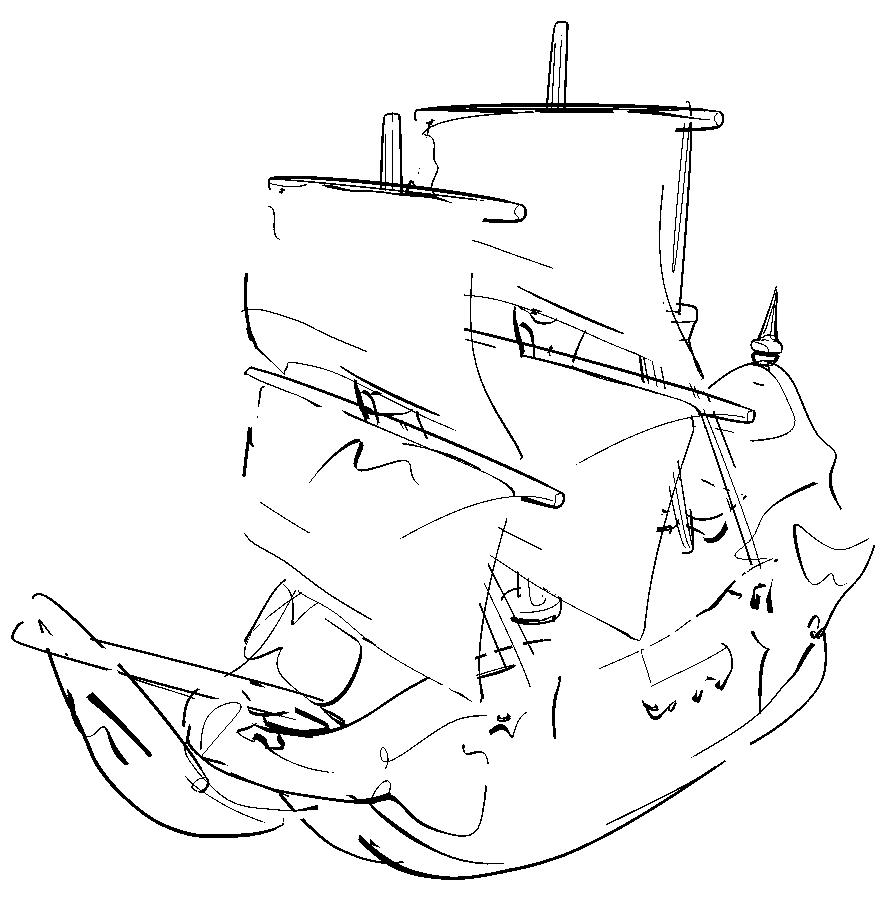
\includegraphics[width=3in]{figs/res/sketch/ship.png}
\caption{
    NPR of a ship model~\cite{Sousa_Przemek_CGF:2003}.
} \label{fig1}
\end{figure}

% ~~~~~~~~~~~~~~~~~~~~~~~~~~~~~~~~~~~~~~~~~~~~~~~~~~
% Figure 4
% ~~~~~~~~~~~~~~~~~~~~~~~~~~~~~~~~~~~~~~~~~~~~~~~~~~

\begin{figure*}[t]
\centering
\begin{tabular} {cccc}
  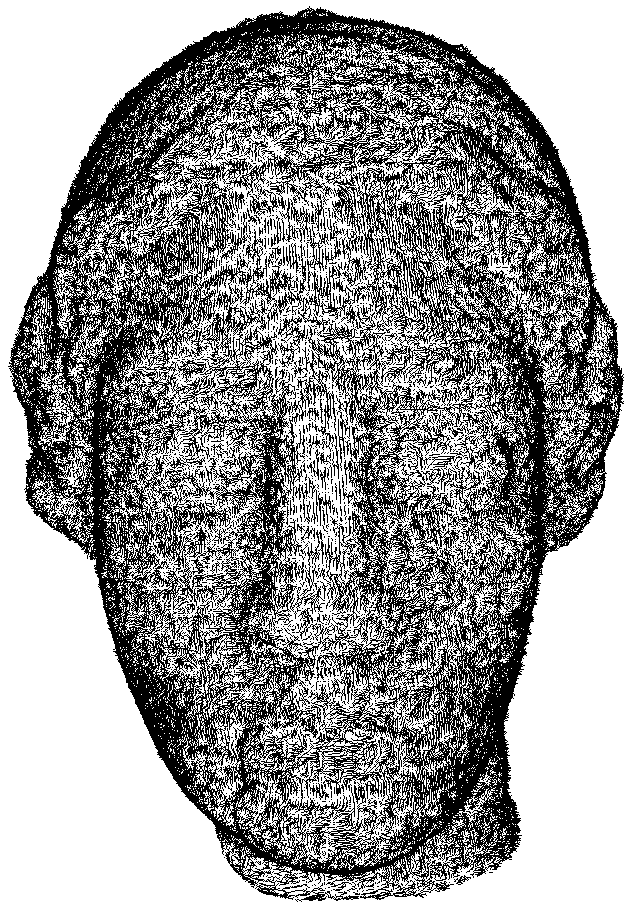
\includegraphics[width=3.5cm]{figs/res/igea/a.png} &
  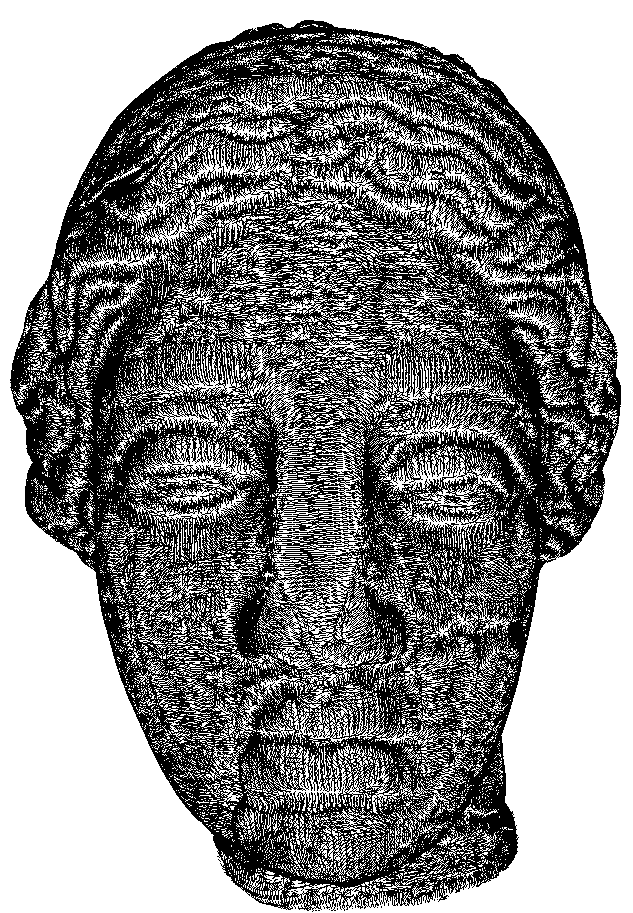
\includegraphics[width=3.5cm]{figs/res/igea/b.png} &
  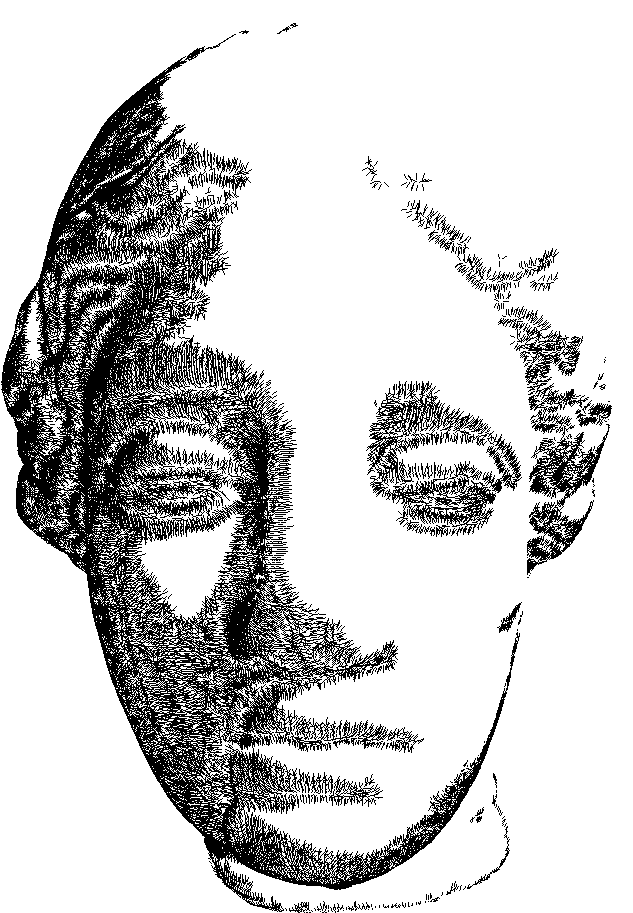
\includegraphics[width=3.5cm]{figs/res/igea/c.png} &
  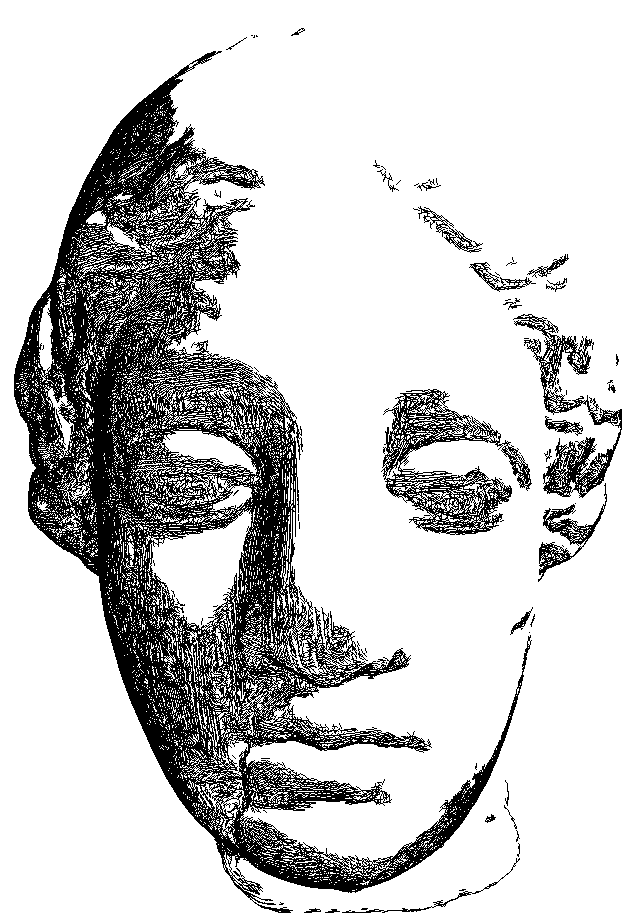
\includegraphics[width=3.5cm]{figs/res/igea/d.png} \\ \\
(a) & (b) & (c) & (d) \\
\end{tabular}
\caption{Here is how to arrange a full row figure using tabular
structure. Also notice that we force it to be at the top of the
page. Results from Sousa et al.~\cite{Sousa_etal_CGI:2004}}
\label{fossil-skull}
\end{figure*}

Your text here...Your text here...Your text here...Your text
here...Your text here... Your text here... Your text here... Your
text here... Your text here... Your text here... Your text
here...Your text here...Your text here...Your text here...Your
text here... Your text here... Your text here... Your text here...
Your text here... Your text here...Your text here...Your text
here... Your text here... Your text here...Your text here... Your
text here... Your text here... Your text here...Your text here...

Your text here...Your text here...Your text here...Your text
here...Your text here... Your text here... Your text here... Your
text here... Your text here... Your text here... Your text
here...Your text here...Your text here...Your text here...Your
text here... Your text here... Your text here... Your text here...
Your text here... Your text here...Your text here...Your text
here... Your text here... Your text here...Your text here... Your
text here... Your text here... Your text here...Your text here...

Your text here...Your text here...Your text here...Your text
here...Your text here... Your text here... Your text here... Your
text here... Your text here... Your text here... Your text
here...Your text here...Your text here...Your text here...Your
text here... Your text here... Your text here... Your text here...
Your text here... Your text here...Your text here...Your text
here... Your text here... Your text here...Your text here... Your
text here... Your text here... Your text here...Your text here...

\acknowledgements{Note there is no section number on the
acknowledgement section header or on the header for the
references.}

%------------------------------------------------------------------
% References
%------------------------------------------------------------------

% To add people to the references without citing them in body
%\nocite{author1995a,author1995b}

\bibliography{refs}

\end{document}
